% !TeX spellcheck = fa-IR
\chapter{نتایج جدید}
\label{chapter:results}
در این فصل ابتدا به بررسی مقاله
\cite{arya}
 می‌پردازیم. این مقاله پایه تحقیقاتی نتایج جدید به دست آمده در این پایان‌نامه است. مزومدار در این مقاله با تعریف مسئله‌ی
\transf{سیستم ذخیره‌سازی توزیع شده با بازیابی محلی تک-شکست}{\SFRDSS: single failure locally recoverable distributed storage system}
اثبات می‌کند این مسئله‌ی دوگان مسئله‌ی کدگذاری اندیس است.

بعد از بررسی کار مزومدار با تعمیم مسئله‌ی سیستم ذخیره‌سازی و معرفی مسئله‌ی
\transf{
	دوگان کدگذاری اندیس منعطف
	}{DPICID: Dual of Pliable Index Coding}
 اثبات می‌کنیم، این مسئله‌ی تعمیم یافته را دوگان 
 \lpicod
  می‌نامیم.
\newpage

\section{
سیستم ذخیره‌سازی توزیع شده با بازیابی محلی تک-شکست \SFRDSS
}
یکی از چالش‌ها در سیستم‌های ذخیره سازی داده توزیع شده، بازیابی داده‌های از دست رفته به دلیل خراب شدن یکی از سرورها است. 
برای حل این مشکل هر داده در چندین سرور ذخیره می‌شود تا در صورت از بین رفتن یکی از سرورها داده‌های آن سرور از دست نرود. چالش این روش هزینه‌ی بازیابی سرور از دست رفته است. یعنی زمانی که سرور خراب شده را جایگزین می‌کنیم و قصد داریم داده‌های سرور قبلی را روی سرور جدید قرار دهیم باید آن داده‌ها را از بقیه سرورهای شبکه 
\transf{دریافت}{download}
کنیم. اما هزینه‌ی دریافت یک داده از سرورهای مختلف متفاوت است.
\say{در سیستم‌های توزیع شده خراب شدن یک تک سرور متداول ترین مشکل است.}

\say{مطالعه‌ی سیستم‌های ذخیره سازی با قابلیت بازیابی اولین بار در
\cite{5550492}
مورد توجه قرار گرفت. در چندین کار جدید این مسیر ادامه پیدا کرد. در
\cite{6259860}
توصیف مناسبی برای
\transf{ویژگی بازیابی محلی}{locally repairable property}
ارائه می‌شود. نتایج این مقاله در جهت‌های مختلف توسعه داده شده است و حتی نتایجی از جنس غیرممکن بودن نیز کشف شده است (برای مثال به
\cite{6570829, kamath2013codes,6818438,silberstein2013optimal, tamo2013optimal}
و به خصوص مقاله اخیر 
\cite{Tamo_2014}
رجوع کنید.). نکته قابل توجه در مقالات بالا عدم توجه به توپولوژی شبکه است و به تمام سرور ها بدون در نظر گرفتن محل فیزیکی آن‌ها، نزدیکی به هم دیگر و ارتباطاتشان با بقیه سرورها نگاه می‌شود.
}
 
 مزومدار در ادامه از یک گراف برای در نظر گرفتن توپولوژی واقعی شبکه استفاده می‌کند. هر رأس متناظر یک سرور است و هر دو سروری که با هم ارتباط دارند با یک یال به یک دیگر متصل شده اند. سپس اثبات می‌کند این مدل جدید دوگان مسئله کدگذاری اندیس است.
 
 \subsection{
 برابری 
 \icod
 و
 \SFRDSS
 }
\label{subsec:arya}
 شبکه‌ی ارتباطی یک سیستم ذخیره سازی توزیع شده را در نظر بگیرید.
 \autoref{fig:storage-graph}
 یک مثال برای چنین شبکه‌ای است. ارتباط بین سرورها بر اساس توانایی ارتباطی آن‌ها است. (که می‌تواند به خاطر فاصله‌ی جغرافیایی، ارتباطات فیبر نوری و
 $\text{\ldots}$
 باشد.) همچنین ممکن است به خاطر مسائل فنی ارتباط سرورها (مثال سرعت متفاوت دانلود و آپلود) از گراف جهت دار استفاده کنیم.
 
 هدف ما این است که اگر یکی از سرورها دچار مشکل شود و دیتای آن از بین برود سرور جایگزین شده در همان نقطه بتواند با گرفتن اطلاعات از سرورهایی که به این نقطه وصل هستند دیتای سرور از دست رفته را بازیابی کند.
 
 پرسش ما این است که با داشتن شبکه‌ی سرورها بیشترین مقدار اطلاعاتی که می‌توان در شبکه ذخیره کرد چقدر است؟
\begin{figure}[H]
	\centering
	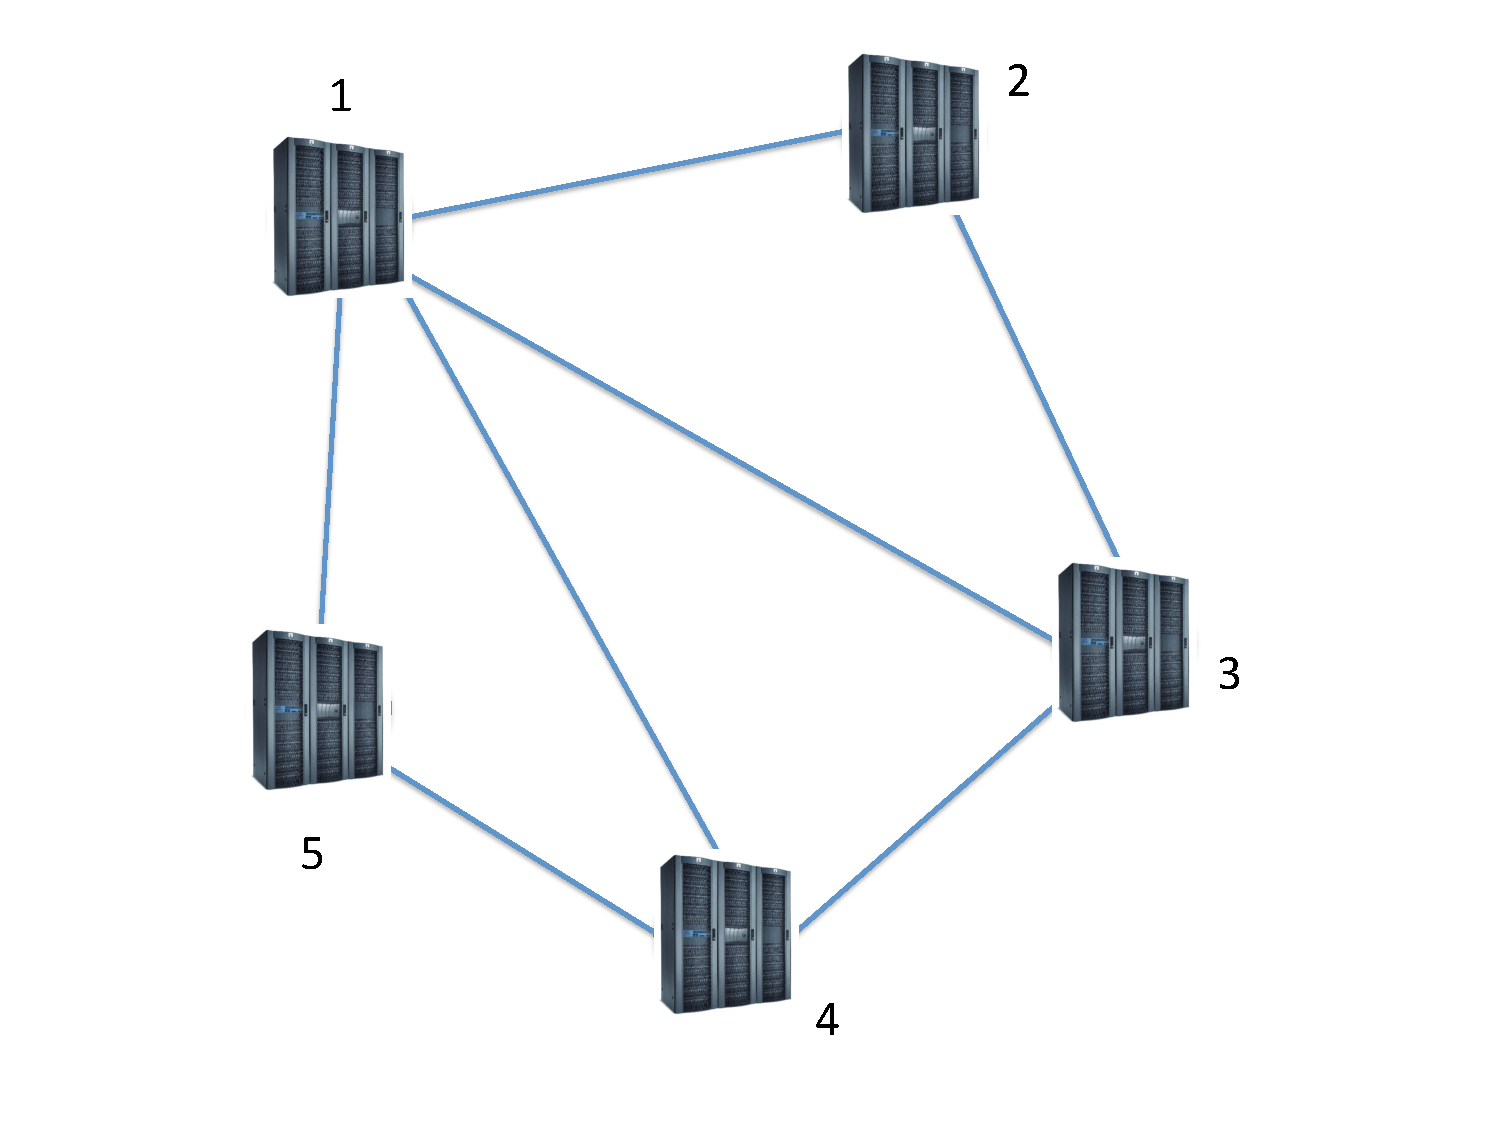
\includegraphics[width=0.5\linewidth]{figs/chapter6/storage-graph}
	\caption[
	مثالی از یک شبکه ارتباطی سرورهای یک سیستم ذخیره‌سازی توزیع شده]{
		مثالی از یک شبکه ارتباطی سرورهای یک سیستم ذخیره‌سازی توزیع شده
		\cite{arya}
		}
	\label{fig:storage-graph}
\end{figure}

\begin{definition}[\transf{
		کد ذخیره‌سازی توزیع‌شده قابل‌بازیابی
	}{RDSS-code}]
	برای میدان
	$\mathbb{F}_{q}$،
	متغیرهای تصادفی
	$X_1, X_2, \ldots, X_n \in \mathbb{F}_{q}$
	و گراف جهت‌دار
	$G = (V, E)$
	که
	$V = [n]$،
		کد ذخیره‌سازی توزیع‌شده قابل‌بازیابی 
		$\mathcal{C} \subseteq \mathbb{F}_{q}$
		،  مجموعه‌ای از بردار‌ها از
		$\mathbb{F}^n_{q}$
		است، همراه با مجموعه‌ی توابع قطعی بازیابی به شکل
		$f_i: \mathbb{F}_q^{\card{N(i)}} \to \mathbb{F}_q$،
		به طوری که برای هر مجموعه از متغیرهای تصادفی 
		$(X_1, X_2,\dots,X_n) \in \mathbb{F}_q^n$
		داشته باشیم:
		$$X_i = f_i(\set{X_j: j \in N(i)}), \quad i = 1,\dots,n$$
\end{definition}

به
$\log_q(\card{C})$
\transf{بُعد کد}{dimension of code}
 گفته می‌شود. برای گراف داده شده‌ی $G$، بزرگترین بعد کد را با
 $\rdss_q(G)$
 نشان می‌دهیم.
  \begin{definition}[مطابقت ماتریس بر \picods]
  	میگوییم ماتریس
  	$A_{n \times n} = (a_{ij}), a_{ij} \in \mathbb{F}_q$
  	بر گراف
  	$G(V, E)$
  	\transf{مطابقت}{fits}
  	می‌کند اگر 
  	\begin{latin}
  		\begin{align*}
  			& \forall i : a_{ii} \ne 0 \\
  			& \forall i \ne j:  (i, j) \notin E \Rightarrow a_{ij} = 0
  		\end{align*}
  	\end{latin}
  \end{definition}
 \begin{definition}[\transf{رتبه کمینه}{minrank}]
	 \label{def:minrank}
 	رتبه کمینه گراف
 	$G$
 	بر روی میدان
 	$\mathbb{F}_q$
 	به صورت زیر تعریف می‌شود:
 	\begin{equation}
 		\minrank_q(G) = \min\set{\rank_{\mathbb{F}_q}(A): A \text{ fits } G}.
 	\end{equation}
 \end{definition}
 \begin{theorem}
	 \label{thm:minranl}
	 اگر طول کد بهینه روی میدان
	 $\fq$
	  در مسئله‌ی کدگذاری اندیس برای گراف
	 $G$
	 را با
	 $\indx_q(G)$
	 نشان دهیم آنگاه داریم:
 	\begin{equation}
 		\indx_q(G) \le \minrank_q(G),
 		\label{eq:bary}
 	\end{equation} 
 \end{theorem}
 \begin{proof}
 		اثبات این قضیه خارج از چارچوب این پایان‌نامه است. برای دیدن اثبات می‌توان به
 	\cite{4031356}
 	رجوع کرد.
 \end{proof}
 \begin{example}[
 	توابع خطی
 	\cite{arya}
 	]
 	برای گراف داده شده در
 	\autoref{fig:storage-graph}
 	داریم:
 	$$
 		N(1) = \set{2,3,4,5}, \, N(2)  = \set{1,3}, N(3)  = \set{1,2,4}, N(4)  = \set{1,3,5},  N(5)  = \set{1,4}
 	$$
 	اگر داده‌ی درون سرور
 	$i$
 	را با
 	$X_i$
 	نشان دهیم برای این‌که بتوانیم در صورت از دست رفتن یک سرور اطلاعات آن را به صورت محلی بازیابی کنیم باید توابع زیر را داشته باشیم: 	
 	$X_1 = f_1(X_2,X_3,X_4,X_5), X_2 = f_2(X_1,X_3), X_3 = f_3(X_1,X_2,X_4), X_4 = f_4(X_1,X_3, X_5), X_5 = f_5(X_1, X_4)$.

 	فرض کنید توابع
 	$f_i$
 	همگی خطی هستند پس برای
 	$\alpha_{ij} \in  \mathbb{F}_q, 1\le i,j\le 5,$
 	خواهیم داشت:
 	 	\begin{align*}
 		X_1 &= \alpha_{12} X_2 +\alpha_{13} X_3 + \alpha_{14}X_4 + \alpha_{15}X_5\\
 		X_2 &= \alpha_{21}X_1+\alpha_{23}X_3\\
 		X_3 &= \alpha_{31}X_1 +\alpha_{32}X_2+\alpha_{34}X_4\\
 		X_4 &= \alpha_{41}X_1 + \alpha_{43}X_3 + \alpha_{45}X_5\\
 		X_5 &= \alpha_{51}X_1+\alpha_{54}X_4.
 	\end{align*}
 	که نتیجه خواهد داد که
 	$(X_1,X_2,\dots, X_5)$
 	در فضای پوچ ماتریس
 	\[
 	D \equiv
 	\left( \begin{array}{ccccc}
 		1 & -\alpha_{12} & -\alpha_{13}  & - \alpha_{14} & -\alpha_{15} \\
 		-\alpha_{21} & 1 &  -\alpha_{23} & 0 & 0 \\
 		-\alpha_{31} & -\alpha_{32} & 1 & -\alpha_{34} & 0\\
 		-\alpha_{41} & 0 &-\alpha_{43}  & 1 & -\alpha_{45}\\
 		-\alpha_{51} &0 & 0 & -\alpha_{54} & 1
 	\end{array} \right).\] 
 	قرار دارد.
 	
 	بعد فضای پوچ ماتریس برابر
 	$\card{\rm{null}(D)} = n - \rank(D)$
 	است. پس اگر خود را به توابع خطی محدود کنیم خواهیم داشت:
 	$$\rdss_q(G) = n - minrank_q(G)$$
 	ولی برای توابع غیر خطی این تساوی برقرار نخواهد بود و خواهیم داشت:
 	\begin{equation}
 		\rdss_q(G) \ge n - \minrank_q(G),
 		\label{eq:minrk}
 	\end{equation}
 	این نامساوی و نامساوی
 	\autoref{eq:bary}
 	این حدس را به ما میدهد که
 	$\rdss_q(G) = n - \indx_q(G)$
 	ولی متأسفانه همان‌طور که در مثال بعدی می‌بینیم این حدس درست نیست.
 \end{example}
 
 \begin{example}[
 	تأثیر توابع غیر خطی
 	\cite{arya}
 	]
 	گراف زیر را در نظر بگیرید:
\begin{figure}[H]
	\centering
	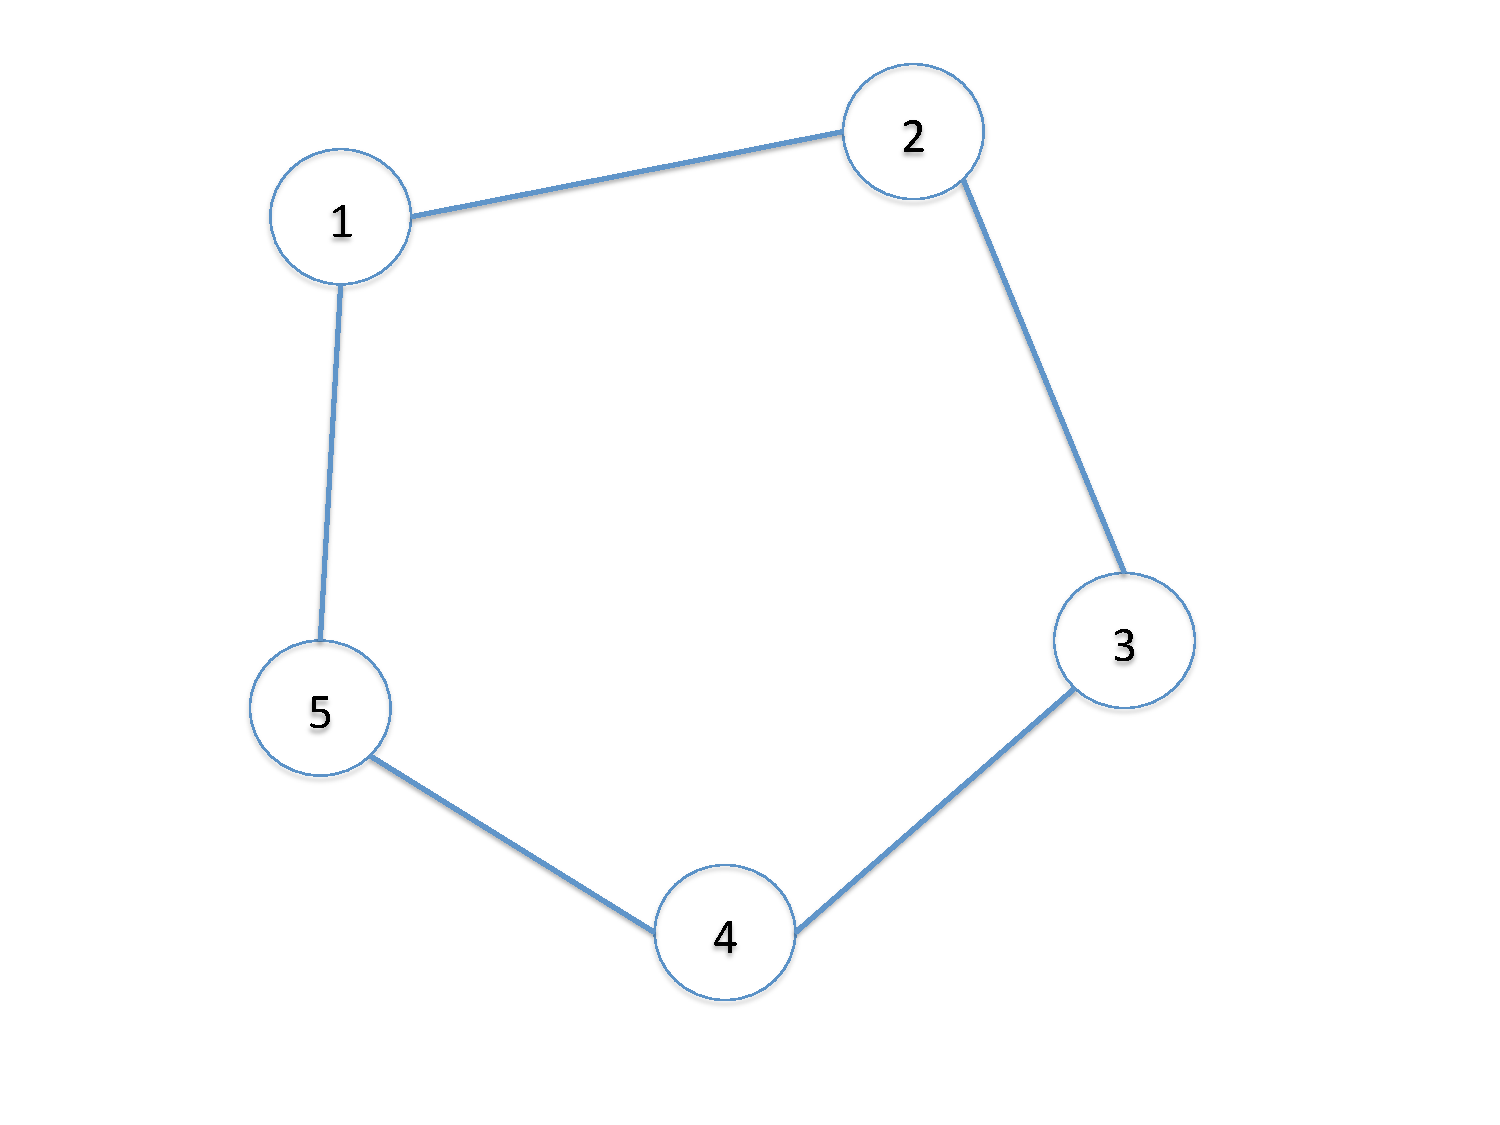
\includegraphics[width=0.4\linewidth]{figs/chapter6/storage-graph-pent}
	\caption[مثال تأثیر توابع غیر خطی]{
		مثال تأثیر توابع غیر خطی
	\cite{arya}
	}
	\label{fig:storage-graph-pent}
\end{figure}
بزرگترین کد برای این گراف به شکل زیر است:
$\set{00000,01100,00011,11011,11101}$
که توابع مربوطه به شکل زیر خواهد بود:
\begin{align*}
	X_1 = X_2 \wedge X_5 \\
	X_2 = X_1 \vee X_3 \\
	X_3 = X_2 \wedge \bar{X}_4 \\
	X_4 = \bar{X}_3 \wedge X_5 \\
	X_5 = X_1\vee X_4
\end{align*}
که نتیجه می‌دهد:
$\rdss_2(G) = \log_2 5$
ولی میدانیم که
$\indx_2(G)=3$.
زیرا اگر فرستنده مقادیر
 $Y_1= X_2+X_3, Y_2= X_4+X_5$ 
 و
  $Y_3= X_1+X_2+X_3+X_4+X_5.$
  را ارسال کند گیرنده‌ها می‌توانند با توابع
  $X_1 = Y_1 + Y_2+Y_3; X_2 = Y_1+X_3; X_3 = Y_1+X_2; X_4 = Y_2+X_5; X_5 = Y_2+X_4$
  پیام‌های خود را بازیابی کنند.
 \end{example}
 
 با وجود آنکه در حالت کلی 
 $\rdss_q(G) \ne n - \indx_q(G)$
 ولی این دو مقدار فاصله‌ی زیادی از هم ندارند. بلکه برای الفباهای با اندازه به اندازه‌ی کافی بزرگ می‌توان آن‌ها را به اندازه‌ی دلخواه به هم نزدیک کرد. این نکته از 
 \autoref{thm:aryamain}
 نتیجه می‌شود.
 \begin{theorem}\label{thm:aryamain}
 	برای گراف
 	 $G(V,E)$,
 	 داریم:
 	\begin{align}
 		n - \rdss_q(G) \le \indx_q(G) \le n -\rdss_q(G) + \log_q\Big(\min\set{n\ln q, 1+ \rdss_q(G)\ln q }\Big)
 	\end{align}
 \end{theorem}
 
 این قضیه در
 \cite{4691014}
 تنها ابزارهای نظریه‌ی گراف اثبات می‌شود. به طور دقیق‌تر، نشان داده می‌شود که اندازه‌ی بزرگترین مجموعه‌ی مستقل در گراف گمراهی
 \autoref{def:confusiongraph}،
 $\gamma(G)$
 برابر طول کد بهینه
$\rdss$
 است و همچنین رابطه‌ی عدد رنگی گراف گمراهی با اندازه‌ی کد
 \icod
 اثبات می‌شود. اثبات اَلون و همکاران از دو نکته استفاده می‌کند. اولاً، عددر نگی گراف نمی‌تواند از عدد رنگی کسری گراف فاصله‌ی زیادی داشته باشد. دوما گراف گمراهی یک گراف
 \transf{رأس ترایا}{vertex transitive}
 است. در نتیجه اندازه‌ی بزرگترین مجموعه‌ی مستقل آن برابر تعداد رأس‌ها تقسیم بر عدد رنگی کسری است.
 
 مزومدار اثباتی بسیار ساده بر مبانی نظریه کدگذاری ارائه می‌دهد که ما نیز در اینجا آن را ذکر می‌کنیم. این قضیه نتیجه‌ی مستقیمی از دو لم
 \autoref{lemma:arya:lem2}
 و
 \autoref{lemma:arya:lem3}
  است. حال به اثبات این دو لم می‌پردازیم.
 \begin{lemma}
 	\label{lemma:arya:lem2}
 	اگر یک کد
 	$\mathcal{C}$
 	با طول
 	$l$
 	برای یک گراف اطلاعات جانبی
 	$G$
 	با
 	$n$
 	رأس وجود داشته باشد، آنگاه یک کد
 	$\rdss$
 	با بُعد
 	$n - l$
 	برای گراف
 	$G$
 	وجود دارد.
 \end{lemma}
 \begin{proof}
 	تابع کدگذاری و تابع‌های کدگشایی کد
 	$\mathcal{C}$
 	را به ترتیب
 	$f: \mathbb{F}_q^n \rightarrow \mathbb{F}_q^l$
 	و
 	$g_i: \mathbb{F}_q^{l + |S_i|} \rightarrow \mathbb{F}_q$
 	می‌گیریم. حتما
 	$y \in \mathbb{F}_q^{l}$
 	وجود دارد که
 	$|\set{x \in \mathbb{F}_q^n: f(x) = y}| \geq q^{n - l}$
 	باشد. حال
 	$D_y \equiv \set{x \in \mathbb{F}_q^n: f(x) = y}$
  	را برابر کد
 	$\rdss$
 	قرار دهید که تابع بازیابی آن عبارت است از:
 	$f_i(\set{X_j, j \in N(i)}) \equiv g_i(y, \set{X_j, j \in N(i)})$
 \end{proof}
 \begin{lemma}
 	\label{lemma:arya:lem4}
 	اگر
 	$\mathcal{C} \subseteq \mathbb{F}_q^n$
 	یک
 	$\rdss$
 	باشد آنگاه هر انتقالی از آن نیز یک کد معتبر خواهد بود. یعنی برای هر
 	$a \in \mathbb{F}_q^n$،
 	$\mathcal{C} + a \equiv \set{y + a: y \in \mathcal{C}}$
 	نیز یک کد معتبر با بعد
 	$\log_q |\mathcal{C}|$
 	خواهد بود.
 \end{lemma}
 \begin{proof}
 	فرض کنید
 	$(x_1, \ldots, x_n) \in \mathcal{C}$.
 	همچنین فرض کنید
 	$a = (a_1, \dots,  a_n)$
 	و
 	$x_i^{'} = x_i + a_i$.
 	طبق فرض تابع بازیابی
 	$f_i$
 	که
 	$x_i = f_i(\set{x_j: j \in N(i)})$
 	وجود دارد. حال تابع بازیابی جدید را به شکل زیر تعریف می‌کنیم:
 	$x_i^{'} = x_i +a_i = f_i(\set{x_j: j \in N(i)}) + a_i \equiv f_i^{'}(\set{x_j^{'}: j \in N(i)})$
 \end{proof}
 ‍\begin{lemma}
 	\label{lemma:arya:lem3}
 	اگر یک کد
 	$\rdss$ $\mathcal{C}$
 	با بعد
 	$k$
 	برای گراف سیستم ذخیره‌سازی
 	$G$
 	با
 	$n$
 	رأس وجود داشته باشد، آنگاه یک کد برای
 	\icodg
 	با طول 
 	$n - k + \log_q(\min{ \{ n \ln q, 1 + k \ln q\}})$
 	وجود دارد.
 \end{lemma}
 \begin{proof}
 	نشان می‌دهیم کدهای
 	$\rdss$،
 	$\mathcal{C}_1, \dots, \mathcal{C}_r: \mathcal{C}_i \in \mathbb{F}_q^n$
 	با بعد
 	$k$
 	وجود دارد که
 	\begin{equation}
 		\bigcup_{i = 1}^r \mathcal{C}_i = \mathbb{F}_q^n
 	\end{equation}
 	و 
 	$r = q^{n - k} \min{n \ln q, 1 + k \ln q}$.
 	برای اثبات وجود این کدها، نشان می‌دهیم که
 	$r$
 	بردار
 	$z_1, \dots, z_r$
 	وجود دارند که
 	\begin{equation}
 		\mathcal{C}_i = \mathcal{C} + z_i \equiv \set{y + z_i: y \in \mathcal{C}}
 	\end{equation}.
 	طبق
 	\autoref{lemma:arya:lem4}
 	تمام کدهای
 	$\mathcal{C}_i$
 	که به شکل بالا تعریف شوند، کدهای
 	$\rdss$
 	با بعد
 	$k$
 	هستند.	 حالا باید $r$ بردار گفته شده را پیدا کنیم. برای این منظور، بردارها را به صورت تصادفی مستقل از فضای برداری
 	$\mathbb{F}_q^n$
 	انتخاب می‌کنیم. برای دو مقدار 
 	$r'$
 	مختلف مسئله را حل می‌کنیم و بین آن‌ها کمینه می‌گیریم.
 	
 	 اگر قرار دهیم
 		$r' = q^{n - k} n \ln q $
 		(به
 		\autoref{thm:vertexx}
 		رجوع کنید)
 	خواهیم داشت:
 	$$Pr(\bigcup_{i = 1}^{r'} \mathcal{C} \ne \mathbb{F}_q^n) \leq  (1 - |\mathcal{C}|/q^n)^{r'}  = \big((1 - \dfrac{1}{q^{n - k}})^{q^{n - k}} \big)^{n \ln q} < q^{-n}$$
 	پس برای احتمال اینکه حداقل یکی از نقاط در پوشش قرار نگیرد داریم:
 	$$q^n * Pr(\bigcup_{i = 1}^{r'} \mathcal{C} \ne \mathbb{F}_q^n) < q^n * q^{-n} \leq 1$$
 	چون احتمال اینکه نقطه‌ای در پوشش قرار نگیرد از یک کمتر است در نتیجه یک انتخاب برای
 	$r'$
 	بردار هست که تمام فضا را بپوشاند.
 	
 	اگر مقدار
 	$r'$
 	را برابر
 	$q^{n - k} k \ln q$
 	قرار دهیم احتمال اینکه کدهای
 	$\mathcal{C}_i$
 	شامل یک نقطه خاص نشوند برابر است با
 	$Pr(\bigcup_{i = 1}^{r'} \ne \mathbb{F}_q^n) \leq q^{- k}$
 	در نتیجه امیدریاضی تعداد کل نقاط خارج از پوشش ایجاد شده توسط
 	$r'$
 	انتقال
 	$\mathcal{C}_1\ldots, \mathcal{C}_{r'}$
 	برابر است با
 	$q^{n - k}$.
 	برای اینکه این نقاط نیز در پوشش ارائه شده قرار گیرند، حداکثر 
 	$q^{n - k}$
 	 انتقال دیگر نیز نیاز داریم که در نهایت به پوششی با حداکثر
 	 $q^{n - k} k \ln q + q^{n - k} = q^{n - k}(k \ln q + 1)$
 	 انتقال می‌رسیم.
 	 
 	  	 با کمینه گرفتن بین دو مقدار بالا به نتیجه مورد نظر می‌رسیم.
 	 
 	 حال توجه کنید که، هر
 	 $y = (y_1, \dots, y_n) \in \mathbb{F}_q^n$
 	 باید عضو حداقل یکی از
 	 $\mathcal{C}_i$ها
 	 باشد. فرض کنید عضو
 	 $\mathcal{C}_i$
 	 باشد. در این صورت تابع کدگذاری برای
 	 \icod
 	 برابر
 	 $f(y) = i$
 	 است. همچنین اگر برای کد
 	 $\mathcal{C}_i$
 	  تابع‌های بازیابی سرور
 	  $j$
 	  ام برابر
 	 $f_j^i$
 	 باشد در این صورت، تابع کدگشایی گیرنده‌ی
 	 $c_i$
 	 در
 	 \icod
 	 برابر
 	 $g_i(i, \set{Y_l: l \in N(j)}) = f_j^i(\set{Y_l: l \in N(j)})$
 	 	خواهد بود.
 	 	واضح است که طول کد 
 	 	\icod
 	 	ارائه شده برابر
 	 	$\log_q(r) = n - k + \log_1(\min{n \ln q, 1 + k \ln q})$
 	 	است.
 \end{proof}
 مزومدار در ادامه اثباتی الگوریتمی دیگری نیز برای همین قضیه ارائه می‌دهد. کاربرد اثبات الگوریتمی در این است که با استفاده از آن می‌توان نشان داد اگر تابع کدگشایی در زمان چندجمله‌ای برای 
 $\rdss$-کد
 $\mathcal{C}$
 وجود داشته باشد، تابع کدگشایی در زمان چندجمله‌ای برای
 \icod
 نیز وجود دارد. از آنجایی که اثبات الگوریتم خارج از چارچوب این پایان‌نامه است برای مطالعه آن به
 \cite{arya}
 رجوع کنید.
 \newpage
\section{نتایج جدید}
\label{sec3}
\subsection{
	دوگانی
	\picod
	 و دوگان کدگذاری اندیس منعطف
}
در این بخش، ابتدا به طور رسمی مسئله دوگان کدگذاری اندیس منعطف را تعریف می‌کنیم. سپس، قضیه اصلی این مقاله را در مورد ارتباط بین مسئله 
\picod
 و دوگان آن بیان می‌کنیم.
\subsubsection{
		دوگان کدگذاری اندیس منعطف
}
\begin{recal}
	دلیل استفاده از واژه‌ی اندیس در نام‌گذاری مسئله کدگذاری اندیس، این است که می‌توان نگاه متفاوتی به مسئله داشت. در نگاه اول، مسئله شامل یک فرستنده و تعدادی گیرنده است که گیرنده‌ها به دنبال داده‌ی جدیدی هستند و وظیفه‌ی فرستنده است که با ارسال پیام‌هایی آن‌ها را آگاه کند. اما نگاه دیگری نیز وجود دارد. در نگاه قبل ما دو عنصر اصلی در مسئله داشتیم: فرستنده و گیرنده‌ها (و البته اطلاعات جانبی گیرنده‌ها). ولی می‌توان خود پیام‌ها را هم به عنوان یک عنصر اصلی در مسئله دید.
	
فرض کنید 
$m$
پیام (متغیر‌ تصادفی) از
$\mathbb{F}_q$
 داریم. قبل از مشخص شدن پیام‌ها، بر اساس گراف اطلاعات جانبی، تعدادی مجموعه به شکل
 $\forall i \in [k]: A_i \subseteq \fq$
 مشخص می‌کنیم که اجتماع آن‌ها کل فضای پیام‌ها را پوشش دهد یعنی:
 $ \bigcup\limits_{i = 1}^k A_i = \fq^m $
 و علاوه بر آن، اگر هر گیرنده بداند پیام‌ها در کدام
 $A_i$
 است بتواند بر اساس اطلاعات جانبی خود پیام مورد نظر خود را بازیابی کند. سپس بعد از مشخص شدن پیام‌ها، فرستنده تنها اندیس مجموعه‌ی شامل پیام را برای گیرنده‌ها ارسال کند. این کار تنها به
 $\log_q(k)$
 ارسال پیام از طرف فرستنده نیاز دارد.
\end{recal}
\begin{example}
	\cite{ourwork}
	فرض کنید پیام‌ها از
	$\mathbb{F}_2$
	می‌آیند یعنی
	$X_i \in \set{0, 1}$
	برای گراف اطلاعات جانبی زیر، کمترین تعداد پیام مورد نیاز برای ارضای همه گیرنده‌ها چند است؟
	\newline
		\begin{minipage}{0.5\textwidth}
				\begin{figure}[H]
					\centering
				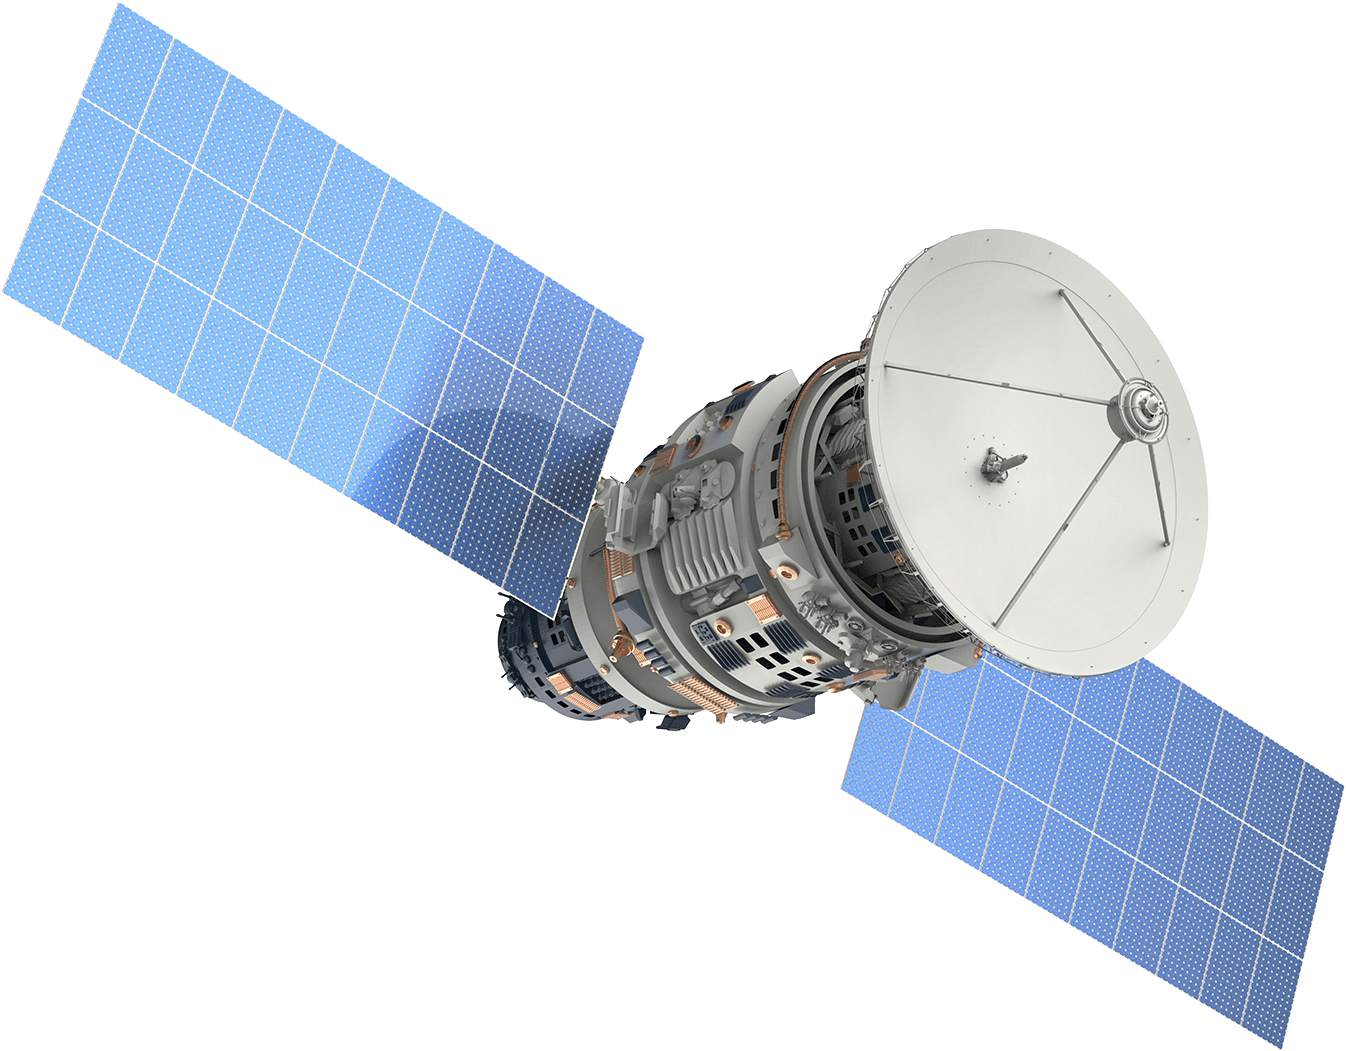
\includegraphics[width=0.3\linewidth]{figs/chapter6/satelite}
			\end{figure}
		\begin{enumerate}
		\item\centering$Y = (X_1,X_2,X_3)$
		\item \centering$Y = (X_1 + X_2 + X_3) $
\end{enumerate}
	\end{minipage}
		\begin{minipage}{0.5\textwidth}
		\centering
		\begin{tikzpicture}[->, >=stealth, auto, semithick]
			% Set the positions of the nodes
			\node[circle, draw=blue, fill=blue!20, inner sep=0pt] (C1) at (0,2) {
					
\includegraphics[width=0.06\linewidth]{figs/chapter6/thinkingemoji.png}
			};
			\node[circle, draw=blue, fill=blue!20, inner sep=0pt] (C2) at (1.5,2) {
					
\includegraphics[width=0.06\linewidth]{figs/chapter6/thinkingemoji.png}
			};
			\node[circle, draw=blue, fill=blue!20, inner sep=0pt] (C3) at (3,2) {
					
\includegraphics[width=0.06\linewidth]{figs/chapter6/thinkingemoji.png}
			};
			\node[above] at (1.5,2.5) {\RL{
				گیرنده‌های جویای دانش!
				}};
			
			
				\node[circle, draw=green, fill=green!20, inner sep=0pt] (B1) at (0,0) {$B_1$};
				\node[circle, draw=green, fill=green!20, inner sep=0pt] (B2) at (1.5,0) {$B_2$};
				\node[circle, draw=green, fill=green!20, inner sep=0pt] (B3) at (3,0) {$B_3$};
				\node[below] at (1.5,-0.5) {\RL{
					دانش لاینفع!
				}};
			
			
				% Draw the edges
				\draw (C1) -- (B1);
			%	\draw[->, color=red]  (C1) -- (B2);
				\draw (C1) -- (B3);
				
				\draw (C2) -- (B1);
				\draw (C2) -- (B2);
			%	\draw[->, color=red]  (C2) -- (B3);
				
		%		\draw[->, color=red]  (C3) -- (B1);
				\draw (C3) -- (B2);
				\draw (C3) -- (B3);
			
			% Position the parts
			\begin{scope}[on background layer]
				\node[fit=(C1) (C2) (C3), draw=blue, fill=blue!10, rounded corners] {};
				\node[fit=(B1) (B2) (B3), draw=green, fill=green!10, rounded corners] {};
			\end{scope}
		\end{tikzpicture}			
	\end{minipage}
	\newline
	 در عکس دو $Y$ ممکن مختلف آمده است. فرستنده می‌تواند در روش اول با سه ارسال نیاز تمام گیرنده‌ها را ارضا کند. در روش دوم تنها با یک ارسال این کار را انجام می‌دهد. زیرا هر گیرنده با استفاده از توابع زیر می‌تواند پیام مورد نظر خود را بازیابی کند:
	\begin{align*}
		\begin{cases}
				X_1 &= Y - X_2 - X_3 \\
				X_2 &= Y - X_1 - X_3  \\
				X_3 &= Y - X_1 - X_2  
			\end{cases}   
	\end{align*}
	با توجه به بحث بالا در مورد نحوه‌ی نگاه به مسئله می‌توان دید که در واقع فرستنده پیام‌ها را به دو دسته تقسیم می‌کند.
		\begin{enumerate}
			\centering
			\item $\set{X: X_1 + X_2 + X_3 = 1}$
			\item $\set{X: X_1 + X_2 + X_3 = 0}$
		\end{enumerate}
	حال هر کدام از گیرنده‌ها بر اساس این‌که پیام در کدام دسته است می‌توانند پیام مورد نظر خود را بازیابی کنند.
\end{example}

همان‌طور که در مثال قبل دیدیم مسئله 
\icod
 را می‌توان به نوعی مسئله‌ی دسته بندی فضای پیام‌ها دید. بر اساس همین ایده، دوگان مسئله کدگذاری  اندیس منعطف را تعریف می‌کنیم. در مسئله دوگان، هیچ فرستنده‌ای وجود ندارد که به گیرنده‌ها بگوید کدام مقدار برای $X$ انتخاب شده است. به جای آن، مجموعه‌ای از بردارهای
  $\mathbb{F}^m$
   وجود دارد که به این مجموعه،
\transf{کتاب کد}{code book}
 (یا 
 \transf{جدول}{table})
 گفته می‌شود که $X$ به آن تعلق دارد. سپس، با توجه به اطلاعات جانبی و کتاب کد، هر گیرنده باید پیام مورد نظر خود را بازیابی کند.
\begin{observation}
	مسئله‌ی دوگان، صورت‌بندی جدیدی از مسئله‌ی کد ذخیره‌سازی توزیع شده قابل‌بازیابی است. مسئله‌ی کد ذخیره سازی را نمی‌توان برای حالت منعطف به صورتی تعمیم داد که هنوز معنادار باشد به همین دلیل از این صورت بندی جدید استفاده می‌کنیم. نتیجه جدید به دست آمده در این پایان‌نامه تعمیم نتیجه مزومدار برای حالت منعطف است.
\end{observation}

\begin{observation}
توجه داشته باشید که در مسئله 
\picods،
هدف کاهش اندازه پیام‌های منتقل شده است در حالی که در مسئله 
\psicod
، هدف افزایش اندازه کتاب کد (جدول قابل استفاده) است.
\end{observation}

\begin{definition}[جدول قابل استفاده]
	\label{def1}
برای یک الفبای داده شده
 $\mathbb{F}$
  و گراف اطلاعات جانبی 
 $G$، 
 یک جدول قابل استفاده 
 $T$
  زیرمجموعه‌ای از 
 $\mathbb{F}^m$ 
 است به طوری که برای هر گیرنده 
 $c_i$
 حداقل یک شاخص 
  $j \in R_i$
  وجود دارد که به ازای تمام اعضای
  $T$
  که با اطلاعات جانبی
  $c_i$
  تطبیق دارند در عضو
  $j$ام
  یکسان باشند. یعنی:
\begin{align*}
    \forall i: \exists j \notin S_i: \forall X, X^\prime: X[S_i] = {X^\prime}[S_i]  \Rightarrow X[j] = {X^\prime}[j]
\end{align*}
ما از اصطلاح جدول استفاده می‌کنیم زیرا عناصر این مجموعه را در یک جدول نمایش می‌دهیم. به این ترتیب، هر ستون یکی از متغیرهای $X_i$ را نشان می‌دهد و هر سطر یک پیام ممکن است.
\end{definition}

مسئله دوگان کدگذاری اندیس منعطف، 
\psicod
، برای یافتن بزرگترین جدول قابل استفاده ممکن برای یک $G$ داده شده است.

\begin{remark}
    ما همیشه می‌توانیم
     $\mathbb{F}^n$ 
     را به جدول‌های قابل استفاده تقسیم کنیم، به عنوان مثال هر 
     $x \in \mathbb{F}^n$ 
     را به عنوان یک جدول قابل استفاده با یک ردیف در نظر بگیریم.
\end{remark}

\begin{lemma}
    برای گراف $G$ و جدول‌های قابل استفاده‌ی
    $T_1, \ldots, T_l \subseteq \mathbb{F}^m$
     که
     $\bigcup\limits_{i} T_i =  \mathbb{F}^m$
     ، یک راه‌حل برای
     \picod
     وجود دارد که تابع رمزگذاری آن عبارت است از تابعی که اندیس جدول قابل استفاده‌ای را ارسال می‌کند که متغیرها از آن انتخاب شده‌اند.
\end{lemma}
\begin{proof}
    گیرنده $c_i$ را در نظر بگیرید. گیرنده 
    $c_i$
    ،
    $X[S_i]$
    را به عنوان اطلاعات جانبی خود دارد. بر اساس تعریف جدول قابل استفاده، شاخص 
    $j \in R_i$
     وجود دارد که
      $c_i$ 
      می‌تواند
      $x_j$
      را بازیابی کند.
\end{proof}

\begin{corollary}
	\label{cor1}
اگر همه حالت‌بندی‌های ممکن برای پیام‌ها (یعنی اعضای مجموعه‌ی
$\mathbb{F}^m$
) را در 
$2^l$ 
جدول قابل استفاده مختلف تقسیم کنیم، آنگاه می‌توانیم فقط با
$l$ 
ارسال، اندیس جدول مورد نظر را برای کاربران ارسال کرده و همه را ارضا کنیم.
\end{corollary}

\begin{note}
    در 
    \lpicod
    ، تابع رمزگذاری 
    $En$
         را می‌توان با یک ماتریس توصیف کرد. اگر فرستنده
    $k$ 
    پیام
     $Y_i = a_{i,1} X_1 + a_{i,2} X_2 \ldots + a_{i,n} X_n$
      را ارسال کند، آنگاه تابع رمزگذاری را می‌توان به شکل زیر نمایش داد.
    \begin{equation*}
        En =
        \begin{pmatrix}
            a_{1,1} & a_{1,2} & \cdots & a_{1,n} \\
            a_{2,1} & a_{2,2} & \cdots & a_{2,n} \\
            \vdots  & \vdots  & \ddots & \vdots  \\
            a_{k,1} & a_{k,2} & \cdots & a_{k,n}
        \end{pmatrix}
    \end{equation*}
\end{note}

\begin{definition}[
	جدول قابل استفاده خطی
	]
	\label{def:lineartable}
    فرض کنید 
    $\mathbb{F}$
     یک میدان متناهی است. یک جدول قابل استفاده 
     $T$ 
     بر روی 
     $\mathbb{F}$
      \textbf{
      خطی
    }
       نامیده می‌شود اگر ردیف‌های 
      $T$ 
      یک فضای برداری بر روی 
      $\mathbb{F}$
       تشکیل دهند.
\end{definition}

مسئله دوگان کدگذاری اندیس منعطف خطی، 
\lpsicod
، یافتن بزرگ‌ترین جدول قابل استفاده خطی ممکن برای گراف اطلاعات جانبی است.

\begin{remark}
    همیشه حداقل یک جدول ممکن خطی وجود دارد، 
    $\set{\overrightarrow{0}}$
    . در حالت خطی، ما می‌توانیم 
    $\mathbb{F}^m$
     را با یک جدول ممکن خطی و هم‌دسته‌های\footnote{\autoref{coset}} آن تقسیم‌بندی کنیم. به سادگی با در نظر گرفتن یک جدول ممکن خطی و تمامی انتقال‌های  آن با بردارهای مختلف این کار قابل انجام است. این کار به ما امکان می‌دهد تا تمام 
     $\mathbb{F}^m$
      را پوشش دهیم.
\end{remark}

\begin{example}
    $G_1$
    و
    $G_2$
    در
    \autoref{figure:example:shit}
     را در نظر بگیرید.
    برای
    $G_1$
    می‌توانیم دسته‌پیام‌ها را در 4 مجموعه مختلف (جدول) تقسیم‌بندی کنیم
    \autoref{figure:example:shittable}
    . در این مثال، همه آن‌ها جدول‌های ممکن هستند. برای
    $G_2$
    ما یک جدول ممکن خطی داریم.این جدول و تنها هم‌دسته آن کل
    $\mathbb{F}_2^3$
    را پوشش می‌دهند.
    \begin{figure}[H]
		\centering
         \begin{subfigure}[b]{0.3\textwidth}
    	         \centering
    \begin{tikzpicture}[->, >=stealth, auto, semithick]
        % Set the positions of the nodes
        \node[circle, draw=blue, fill=blue!20, inner sep=0pt] (C1) at (0,2) {$C_1$};
        \node[circle, draw=blue, fill=blue!20, inner sep=0pt] (C2) at (1.5,2) {$C_2$};
        \node[circle, draw=blue, fill=blue!20, inner sep=0pt] (C3) at (3,2){$C_3$};
        \node[circle, draw=green, fill=green!20, inner sep=0pt] (B1) at (0,0) {$B_1$};
        \node[circle, draw=green, fill=green!20, inner sep=0pt] (B2) at (1.5,0) {$B_2$};
        \node[circle, draw=green, fill=green!20, inner sep=0pt] (B3) at (3,0) {$B_3$};
        % Draw the edges
        \draw (C1) -- (B2);
        \draw (C1) -- (B3);
        \draw (C2) -- (B1);
        \draw (C2) -- (B3);
        \draw (C3) -- (B1);
        \draw (C3) -- (B2);
        % Position the parts
        \begin{scope}[on background layer]
            \node[fit=(C1) (C2) (C3), draw=blue, fill=blue!10, rounded corners] {};
            \node[fit=(B1) (B2) (B3), draw=green, fill=green!10, rounded corners] {};
        \end{scope}
    \end{tikzpicture}
        \caption{$G_2$}
             \end{subfigure}
                 \begin{subfigure}[b]{0.3\textwidth}
        	\centering
     \begin{tikzpicture}[->, >=stealth, auto, semithick]
    	% Set the positions of the nodes
    	\node[circle, draw=blue, fill=blue!20, inner sep=0pt] (C1) at (0,2) {$C_1$};
    	\node[circle, draw=blue, fill=blue!20, inner sep=0pt] (C2) at (1.5,2) {$C_2$};
    	\node[circle, draw=blue, fill=blue!20, inner sep=0pt] (C3) at (3,2){$C_3$};
    	\node[circle, draw=green, fill=green!20, inner sep=0pt] (B1) at (0,0) {$B_1$};
    	\node[circle, draw=green, fill=green!20, inner sep=0pt] (B2) at (1.5,0) {$B_2$};
    	\node[circle, draw=green, fill=green!20, inner sep=0pt] (B3) at (3,0) {$B_3$};
    	% Draw the edges
    	\draw (C1) -- (B2);
    	\draw (C1) -- (B3);
    	\draw (C2) -- (B1);
    	\draw (C3) -- (B2);
    	% Position the parts
    	\begin{scope}[on background layer]
    		\node[fit=(C1) (C2) (C3), draw=blue, fill=blue!10, rounded corners] {};
    		\node[fit=(B1) (B2) (B3), draw=green, fill=green!10, rounded corners] {};
    	\end{scope}
    \end{tikzpicture}
    \caption{$G_1$}
       \label{figure:example:shit}
            \end{subfigure}
                    \caption{مثال گراف اطلاعات جانبی برای جدول قابل استفاده}
            \label{fig:three graphs}
       	\end{figure}
       	
       	\begin{table}[H]
       		    \begin{subtable}[h]{0.45\textwidth}
       			\centering
	        		\begin{tabular}{|c|}
	        			\hline
	        			000 \\
	        			\hline
	        			001 \\
	        			\hline
	        		\end{tabular}
	        		\caption{$T_1$}
	        		\end{subtable}
	        		       		    \begin{subtable}[h]{0.45\textwidth}
	        			\centering
	 		       		\begin{tabular}{|c|}
	 		       			\hline
	 		       			000  \\
	 		       			\hline
	 		       			011   \\
	 		       			\hline
	 		       			110  \\
	 		       			\hline
	 		       			101   \\
	 		       			\hline
	 		       		\end{tabular}
	 		       	\caption{$T_2$}
       	       \label{figure:example:shittable}
       	       	        		\end{subtable}
       	       	        		\caption{مثالی از جدول‌های قابل استفاده}
      	\end{table}
\end{example}

\begin{lemma}
    فرض کنید 
    $G$ 
    یک گراف دوبخشی با بخش‌های
    $C$
    و
    $B$
     باشد. اگر 
    $(En, I, \overrightarrow{f})$
    یک اندیس‌کد قابل انعطاف خطی برای 
    $G$
     باشد، آنگاه یک 
     \lpsicod،
     مانند
      $(W, J, \overrightarrow{g})$
     وجود دارد به طوری که 
     $W  = ker(En)$.
\end{lemma}

\begin{proof}
    ابتدا ایده اثبات را مرور می‌کنیم. برای هر 
    \lpicod
    ترکیب‌های خطی که سرور به کاربران ارسال می‌کند را در نظر بگیرید. ضرایب این ترکیب‌ها، یک جدول قابل استفاده‌ی خطی را تشکیل می‌دهند.
حال
    \lpsicod
    را با پارامترهای
    $(W, J, \overrightarrow{g})$
     به شکل زیر تعریف می‌کنیم:
     $$W = ker(En), \overrightarrow{g}_i = \overrightarrow{f}_i(\overrightarrow{0}, X[S_i]), J = I$$
    $\sspan(W)$
     را در نظر بگیرید. اگر بردار پیام‌های
     $X$
      از این فضای برداری باشد، آنگاه پیام ارسالی توسط فرستنده بردار تمام صفر خواهد بود چون 
      $En \times X = \overrightarrow{0}$.
      چون
      $X \in \sspan(W)$
       بردار ارسال شده توسط فرستنده برابر
      $\overrightarrow{0}$
       است و از آنجایی که کاربر 
       $i$-ام
        می‌تواند 
       $X[I_i]$
        را در 
        \picod
         حدس بزند، می‌تواند
         $\overrightarrow{f}_i$ 
        را با 
        $\overrightarrow{0}$ 
        به عنوان کد ارسالی به عنوان تابع رمزگشایی خود استفاده کند. پس 
        $\sspan(W)$
         یک جدول قابل استفاده‌ی خطی تشکیل می‌دهد و 
        $(W, J, \overrightarrow{g})$ 
        یک راه‌حل است.
\end{proof}

\begin{lemma}
    اگر
     $(W, J, \overrightarrow{g})$
      یک 
      \lpsicod
       برای $G$ باشد، آنگاه یک
       \lpicod
        $(En, I, \overrightarrow{f})$
        وجود دارد به طوری که
         $\sspan(En) = W^{\bot}$
\end{lemma}

\begin{proof}
    فرض کنید 
    $r = dim(W)$
     و 
     $\set{V_1, V_2, \ldots, V_{n - r} }$
     یک پایه برای فضای
      $n - r$
       بعدی 
      $W^\bot$
       باشد. ماتریس کدگذاری 
      $En$
       را به عنوان یک ماتریس 
     $(n - r) \times n $
      تعریف کنید که سطرهای آن 
      $V_1, V_2, \ldots, V_{n - r}$
       هستند. واضح است که 
      $\sspan(En) = W^\bot$.
       همچنین 
       $J = I$ 
       . قرار دهید
       $$\overrightarrow{f}_i(\overrightarrow{R}, En(X[S_i]) = f(En(X[S_i] - R[S_i])) + R[I_i]: st.\exists! V \in W: V + R = X $$
      اکنون باید اثبات کنیم که کاربر $i$-ام می‌تواند $X[I_i]$ را در هر انتخابی برای بردار پیام‌ها بازیابی کند. به بیان دیگر، بردارهای پیام متفاوتی وجود ندارند که در 
    $X[I_i]$‌
    متفاوت باشند و در عین حال در
    $X[S_i]$
      و کد ارسالی($En(X)$) یکسان باشند.
       
       فرض کنید خلاف این حکم برقرار است. آنگاه 
     $X_1, X_2, i$
      وجود دارد به طوری که 
     $En(X_1) = En(X_2)$
      و 
     $X_1[S_i] = X_2[S_i]$
      اما 
     $X_1[I_i] \neq X_2[I_i]$.
     اگر 
     $W_1, \ldots, W_t$
      هم‌دسته‌های 
     $W$
      باشند آنگاه بردارهای یکتایی وجود دارد که 
     $X_1 = V_1 + {V^\prime}_1, X_1 = V_2 + {V^\prime}_2$
     ، که در آن 
     $V_1, V_2 \in W$
      و 
      $V^\prime_1 \in W_p, V^\prime_2 \in W_q$.
    بر اساس تعریف جدول قابل استفاده، داریم
     $En(V_1) = En(V_2) = 0$.
    
    چون پیام ارسالی فرستنده یکسان است
    $En(X_1) = En(X_2)$
    پس
    $X_1$ و $X_2$
     از یک زیرمجموعه هستند، یعنی 
    $V^\prime_1 = V^\prime_2$
    .
    
    ما ادعا می‌کنیم که برای هر دو زیرمجموعه متفاوت 
    $W_1$ و $W_2$
     داریم: 
    $$\forall U_1, U_2: U_1 \in W_1, U_2 \in W_2: En(U_1) \neq En(U_2)$$
    اگر این ادعا برقرار باشد کاربران می‌توانند بردار پیام را از همه بردارهای پیام دیگر تمیز دهند. فرض کنید 
    $W_j$ 
    زیرمجموعه‌ای باشد که 
    $X_1$ و $X_2$
     در آن قرار دارند، آنگاه: 
     $R = U - U^\prime: U, U^\prime \in W_j$. 
     حال، 
     $X_1 - R$ و $X_2 - R$ 
     هر دو در 
     $W$
      قرار دارند پس کاربر می‌تواند بین آنها تمایز قائل شود. اما این یک تناقض است زیرا پس از اضافه کردن 
     $R[I_i]$
      به پیام 
     $X[I_i]$،
     کاربر 
     $i$-ام
      می‌تواند بین 
      $X_1$ و $X_2$ 
      تمایز قائل شود.
     
    حال کافی است تا ادعا را ثابت کنیم. فرض کنید ادعا برقرار نباشد. از آنجایی که $En$ خطی است، داریم: 
    $$En(U_1) = En(U_2) \Rightarrow En(U_1 - U_2) = 0 \Rightarrow U_1 - U_2 \in W \Rightarrow \exists i: U_1, U_2 \in W_i$$
    اما ما فرض کرده بودیم که
     $W_1 \neq W_2$
     .
\end{proof}

\begin{theorem}
    \label{thm1}
    برای هر گراف اطلاعات جانبی 
    $G$، 
    \lpsicod
    با پارامترهای
     $(W, J, \overrightarrow{g})$
     دوگان جبری خطی
      \lpicod
      با پارامترهای
       $(En, I, \overrightarrow{f})$ 
      است به این معنا که:
    \begin{align*}
    (W, J, \overrightarrow{g}) &= \begin{cases}
                                      W = ker(En)\\
                                      I = J \\
                                      \overrightarrow{g}_i(En(X[S_i])) = \overrightarrow{f}_i(\overrightarrow{0}, En(X[S_i])\\
    \end{cases} \\
    (En, I, \overrightarrow{f}) &= \begin{cases}
                                       \sspan(En) = W^{\bot} \\
                                       J = I \\
                                       \overrightarrow{f}_i(\overrightarrow{R}, En(X[S_i]) = g(En(X[S_i] - R[S_i])) + R[I_i]: \exists! V \in W: V + R = X \\
    \end{cases}
    \end{align*}
    و 
    $dim(W) = n - dim(En)$.
     یعنی اگر
     $En: \mathbb{F}^n \rightarrow \mathbb{F}^k$
      و جدول قابل استفاده
      $W$
       دارای 
       $l$
       بردار پیام باشد پس 
       $\log(l) + k = n$.
\end{theorem}
\begin{proof}
    این گزاره نتیجه‌ی دو لم آخر است. تنها کافی است برابری ابعاد را نشان دهیم. که از تساوی جبرخطی
    $dim(W) + dim(W^{\bot}) = n$ 
    نتیجه می‌شود.
\end{proof}

حال می‌خواهیم برای حالت غیر خطی مشابه قضیه
 \autoref{thm:aryamain}
برای مسئله
\picod
نتایجی به دست آوریم. مشابه
 \autoref{lemma:arya:lem2}
 لم زیر را داریم.
\begin{lemma}
	\label{lamma:our:lemma2}
	اگر
	$C$
	یک \picod با طول
	$l$
	باشد، آنگاه یک جدول شدنی
	$T$
	با اندازه‌ی
	$|T| = q^{n - l}$
	برای گراف
	$G$
	وجود دارد.
\end{lemma}
\begin{proof}
	اثبات کاملا مشابه اثبات
	\autoref{lemma:arya:lem2}
	است. تابع کدگذاری و تابع‌های کدگشایی کد
	$\mathcal{C}$
	را به ترتیب
	$f: \mathbb{F}_q^n \rightarrow \mathbb{F}_q^l$
	و
	$g_i: \mathbb{F}_q^{l + |S_i|} \rightarrow \mathbb{F}_q$
	می‌گیریم. حتما
	$y \in \mathbb{F}_q^{l}$
	وجود دارد که
	$|\set{x \in \mathbb{F}_q^n: f(x) = y}| \geq q^{n - l}$
	باشد. حال
	$D_y \equiv \set{y \in \mathbb{F}_q^n: f(y) = x}$
	را برابر کد
	$\rdss$
	قرار دهید که تابع بازیابی آن عبارت است از:
	$f_i(\set{X_j, j \in N(i)}) \equiv g_i(y, \set{X_j, j \in N(i)})$.
\end{proof}
مشابه
\autoref{lemma:arya:lem4}
نیز، لم زیر برقرار است.
\begin{lemma}
	\label{lemma:our:lemma4}
	اگر
	$T$
	یک جدول شدنی با اندازه‌ی
	$|T|$
	 برای 
	\psicod
	باشد، هر انتقالی از آن نیز یک جدول شدنی برای
	\psicod
	با اندازه‌ی $|T|$ است. به بیان دیگر، برای هر بردار
	$a \in \mathbb{F}_q^n$
	جدول
	$T + a = \set{t + a: T \in T}$
	نیز یک جدول شدنی است.
\end{lemma}
\begin{proof}
	اثبات مشابه اثبات
	\autoref{lemma:arya:lem4}
	است.
	فرض کنید
	$(x_1, \ldots, x_n) \in \mathcal{C}$.
	همچنین فرض کنید
	$a = (a_1, \dots,  a_n)$
	و
	$x_i^{'} = x_i + a_i$.
	طبق فرض تابع بازیابی
	$f_i$
	که
	$x_i = f_i(\set{x_j: j \in N(i)})$
	وجود دارد. حال تابع بازیابی جدید را به شکل زیر تعریف می‌کنیم:
	$x_i^{'} = x_i +a_i = f_i(\set{x_j: j \in N(i)}) + a_i \equiv f_i^{'}(\set{x_j^{'}: j \in N(i)})$
\end{proof}
در نهایت، مشابه
\autoref{lemma:arya:lem3}
نیز لم زیر برقرار است.
\begin{lemma}
	\label{lemma:our:lemma3}
	اگر
	$T$
	یک جدول شدنی با اندازه‌ی
	$q^k$
	برای 
	\psicod
	روی گراف
	$G$
	باشد، آنگاه یک کد
	$C$
	برای
	\picod
	روی 
	$G$
	با طول حداکثر
	$n - k + \log(\min{ \{n \ln q, 1 + k \ln q \} })$
	وجود دارد.
\end{lemma}
\begin{proof}
	اثبات مشابه اثبات
	\autoref{lemma:arya:lem3}
	است.
	
	نشان می‌دهیم جدول‌های شدنی
	$T_1, \ldots, T_r \in \mathbb{F}_q^m$
	با بعد
	$k$
	وجود دارد که
	\begin{equation}
		\bigcup_{i = 1}^r \mathcal{C}_i = \mathbb{F}_q^m
	\end{equation}
	و 
	$r = q^{n - k} \min{ \{n \ln q, 1 + k \ln q\}} $.
	برای اثبات وجود این جدول‌ها، نشان می‌دهیم که
	$r$
	بردار
	$z_1, \dots, z_r$
	وجود دارند که
	\begin{equation}
		T_i = T + z_i \equiv \set{y + z_i: y \in T}
	\end{equation}
	طبق
	\autoref{lemma:our:lemma4}
	تمام جدول‌های
	$T_i$
	که به شکل بالا تعریف شوند، جدول‌های شدنی	با بعد
	$k$
	هستند.	 حالا باید $r$ بردار گفته شده را پیدا کنیم. برای این منظور، بردارها را به صورت تصادفی و مستقل از فضای برداری
	$\mathbb{F}_q^n$
	انتخاب می‌کنیم. برای بردار تصادفی
	$z_i$
	احتمال اینکه 
	$x \in \mathbb{F}_q^n$
	در
	$T + z_i$
	نباشد برابر
	$ (1 - |T|/q^n)$
	است. حال برای دو مقدار مختلف
	$r$
	مسئله را حل می‌کنیم.
	 اگر مقدار
	$r$
	را برابر
	$r = q^{n - k} n \ln q $
	قرار دهیم، احتمال اینکه یک
		$x \in \mathbb{F}_q^n$
	وجود داشته باشد که در اجتماع این جدول‌ها نباشد برابر است با:
		\begin{equation}
			Pr(\bigcup_{i = 1}^{r} \mathcal{C} \ne \mathbb{F}_q^n) \leq  (1 - |\mathcal{C}|/q^n)^{r}  = \big((1 - \dfrac{1}{q^{n - k}})^{q^{n - k}} \big)^{n \ln q} < q^{-n}
			\end{equation}
	پس برای احتمال اینکه حداقل یکی از نقاط در پوشش قرار نگیرد داریم:
	$$q^n * Pr(\bigcup_{i = 1}^{r} \mathcal{C} \ne \mathbb{F}_q^n) < q^n * q^{-n} \leq 1$$
	چون احتمال اینکه نقطه‌ای در پوشش قرار نگیرد از یک کمتر است در نتیجه یک انتخاب برای
	$r$
	بردار هست که تمام فضا را بپوشاند.
	
	اگر مقدار
	$r$
	را برابر
	$q^{n - k} k \ln q$
	قرار دهیم احتمال اینکه جدول‌های
	$T_i$
	شامل یک نقطه خاص نشوند برابر است با
	$Pr(\bigcup_{i = 1}^{r} \ne \mathbb{F}_q^n) \leq q^{- k}$.
	در نتیجه امیدریاضی تعداد کل نقاط خارج از پوشش ایجاد شده توسط
	$r$
	انتقال
	$T_1, \ldots, T_r$
	برابر است با
	$q^{n - k}$.
	برای اینکه این نقاط نیز در پوشش ارائه شده قرار گیرند، حداکثر 
	$q^{n - k}$
	انتقال دیگر نیز نیاز داریم که در نهایت به پوششی با حداکثر
	$q^{n - k} k \ln q + q^{n - k} = q^{n - k}(k \ln q + 1)$
	انتقال می‌رسیم.		 	  	 
	با کمینه گرفتن بین دو مقدار بالا به نتیجه مورد نظر می‌رسیم.
	
	حال توجه کنید که، هر
	$w = (w_1, \dots, w_n) \in \mathbb{F}_q^n$
	باید عضو حداقل یکی از
	$T_i$ها
	باشد. فرض کنید عضو
	$T_i$
	باشد. در این صورت تابع کدگذاری
	\picod
	برابر
	$f(w)) = i$
	است. همچنین اگر برای جدول
	$T_i$
	تابع بازیابی برای گیرنده‌ی
	$j$
	ام برابر
	$f_j^i$
	باشد در این صورت، تابع کدگشایی گیرنده‌ی
	$c_j$
	در
	\picod
	برابر
	$g_j(i, w[S_j]) = f_j^i(s[S_j])$
	خواهد بود.
	واضح است که طول کد 
	\picod
	ارائه شده برابر
	$\log_q(r) = n - k + \log_1(\min{n \ln q, 1 + k \ln q})$
	است.
\end{proof}
\begin{theorem}
	\label{thm:ourmain}
	برای گراف
	$G(V,E)$,
	داریم:
	\begin{multline}
		n - \psindx_q(G) \le \pindx_q(G) \\ \le n -\psindx_q(G) + \log_q\Big(\min\set{n\ln q, 1+ \psindx_q(G)\ln q }\Big)
	\end{multline}
\end{theorem}
\begin{proof}
	این قضیه نتیجه‌ی مستقیم
	\autoref{lemma:our:lemma3}
	و
	\autoref{lamma:our:lemma2}
	است.
\end{proof}

\subsection{
	مثال سخت
}
\transf{مثال سخت}{hard example}
در 
\autoref{thm:hardexam1}
با یک مثال سخت برای حالت خطی آشنا شدیم. در این بخش یک مثال سخت برای حالت کلی ارائه می‌دهیم و رابطه‌ای بین اندازه جدول قابل استفاده و طول کد می‌یابیم.

برای این مثال از میدان 
$\mathbb{F}_2$
استفاده می‌کنیم.

\begin{definition}[	بردار مشخصه اطلاعات جانبی	]
	برای گراف اطلاعات جانبی (چه در مسئله‌ی
	\picod
	و چه در مسئله‌ی دوگان) روی میدان
	$\mathbb{F}_2$
	برای گیرنده‌ی 
	$c_i$
	با اطلاعات جانبی
	$S_i$
	بردار مشخصه اطلاعات جانبی آن را به صورت زیر تعریف می‌کنیم.
	\begin{align}
		C_i =
		\begin{cases}
			\begin{array}{ll}
			1 & i \in S_i \\
			0 &  i \in R_i
		\end{array}
		\end{cases}
	\end{align}
	یا به طور مشابه
	$C_i[S_i] = \vec{1}$
	و
	$ C_i[R_i] = \vec{0}$
	همچنین تعریف می‌کنیم
	$\setcomp{C_i} = \vec{1} + C_i$
\end{definition}

\begin{lemma}
	\label{lemma:tableconstraint}
	فرض کنید
	$T$
	یک جدول قابل استفاده برای گراف اطلاعات جانبی
	$G$
	باشد که شامل
	$\card{T}$
	بردار پیام است. برای بردارهای مشخصه‌ی اطلاعات جانبی
	$C = \set{C_1, \ldots, C_n}$
	داریم:
	\begin{align}
		\forall i \in [n]: \nexists j, k \in [\card{T}]: T_j + T_k = \setcomp{C_i}
	\end{align}
\end{lemma}
\begin{proof}
	ابتدا توجه کنید که
	$T_j + T_k = \setcomp{C_i}$
	به چه معنی است. اگر درایه‌ی
	$r$-ام
	در
	$\setcomp{C_i}$
	یک باشد یعنی گیرنده‌ی
	$i$-ام
	با بازیابی پیام
	$r$-ام
	ارضا می‌شود. از طرفی وقتی همین درایه در
	$T_j + T_k$
	یک باشد به این معنی است که مقدار آن در دو پیام متفاوت است. برعکس، اگر درایه‌ی 
	$r$-ام
	در
	$\setcomp{C_i}$
	صفر باشد یعنی گیرنده‌ی $i$-ام
	مقدار پیام
	$r$-ام
	را در اطلاعات جانبی خود دارد در حالی که وقتی همین درایه در
	$T_j + T_k$
	صفر باشد به این معنی است که مقدار آن در دو پیام یکسان است. یعنی عملا پیام‌هایی که برای گیرنده‌ی
	$i$-ام
	ارزش دارند در دو پیام متفاوت اند و پیام‌هایی که در اطلاعات جانبی دارد در دو پیام یکسان اند.
	
	حال همین ایده را به صورت رسمی طرح می‌کنیم. از برهان خلف استفاده می‌کنیم. اگر
	$i$
	،
	$j$
	و
	$k$
	با شرایط گفته شده وجود داشته باشند، در این صورت گیرنده‌ی
	$c_i$
	بین بردارهای پیام
	$T_i$
	و
	$T_j$
	نمی‌تواند تفاوتی قائل شود زیرا
	$(T_i + T_j)[S_i] = \setcomp{C_i}[S_i] = \vec{0}$
	یعنی چون این حاصل جمع در
	$\mathbb{F}_2$
	انجام می‌شود، تک تک درایه‌های این دو بردار برابر هستند. پس اطلاعات جانبی
	$c_i$
	روی این دو بردار پیام یکسان است. اما از طرفی
	$(T_i + T_j)[R_i] = \setcomp{C_i}[R_i] = \vec{1}$
	و این یعنی تمام پیام‌هایی که خارج از اطلاعات جانبی
	$c_i$
	هستند در این دو پیام متفاوت‌اند و در نتیجه این گیرنده بین این دو پیام نمی‌تواند تفاوتی قائل شود و جدول
	$T$
	یک جدول قابل استفاده نیست که خلاف فرض اولمان است.
\end{proof}
\begin{remark}
توجه کنید که در استدلال بالا استفاده‌ای از خطی بودن یا نبودن کد نکردیم. این نکته از آن جهت حائز اهمیت است که در قضیه‌های بعد شرطی روی خطی بودن کد برای کران ارائه شده نداریم.
\end{remark}
\begin{definition}[گراف سخت]
	\label{def:our:linearspacepicod}
	 یک زیر فضای خطی 
	$n$
	بعدی از
	$\mathbb{F}^m_2$
	در نظر بگیرید.
	$n$
	بردار پایه
	$V_1, \ldots, V_n$
	برای آن در نظر بگیرید. این 
	$k$
	بردار را بردارهای مشخصه‌ی اطلاعات جانبی 
	$n$
	گیرنده‌ی مسئله در نظر بگیرید یعنی
	$C_i = V_i$.
	این یک نمونه از مسئله
	\picod
	روی میدان
	$\mathbb{F}_2$
	با
	$n$
	گیرنده و 
	$m$
	پیام است که به آن مسئله‌ی 
	\picod
	با اطلاعات جانبی ساخته شده از یک زیر فضای خطی
	$n$
	بُعدی می‌گوییم.
\end{definition}

\begin{theorem}
	\label{thm:our:hardexample}
	برای هر  جدول قابل استفاده
	مانند
	$T$
	 در مسئله‌ی دوگان برای مسئله‌ی
	\picod
	با اطلاعات جانبی ساخته شده از یک زیر فضای خطی
	$n$
	بعدی داریم:
	\begin{align*}
		\card{T} \leq 2^{m - n}
	\end{align*}
\end{theorem}
\begin{proof}
	طبق
	\autoref{lemma:tableconstraint}
	هیچ دو بردار پیام
	$T_1$
	و
	$T_2$
	وجود ندارند که
	$T_1 + T_2 \in C$
	پس مجموعه‌های
	$T_i + C$
	از هم‌دیگر مجزا اند یعنی
	$\forall i, j \in [\card{T}]: T_i + C \cap T_j + C = \emptyset$.
 پس چون
	$\card{T_i + C} = \card{C}$
	داریم
	\begin{align}
	T + C =  \bigcup_{i \in [\card{T}]} \card{T_i} + C \subseteq \mathbb{F}_2^m \Rightarrow \card{T + C} = \card{T } * \card{C} \leq 2^m \Rightarrow \card{T} \leq 2^{m - n}
		\end{align}
\end{proof}

همان‌طور که پیش از این گفته شد در استدلال قبل از خطی بودن کد استفاده‌ای نکردیم. بلکه از خطی بودن اطلاعات جانبی استفاده کردیم. به طور مشابه وقتی جدول نیز خطی باشد می‌توانیم حکم زیر را ثابت کنیم.
\begin{theorem}
	اگر 
	$T$
	یک 
	\nameref{def:lineartable}
	باشد، در این صورت
	$T \cap \setcomp{C} = \emptyset$.
\end{theorem}
\begin{proof}
	چون
	$T$
	یک جدول قابل استفاده‌ی خطی است، پس
	$\forall i, j: \exists k: T_i + T_j = T_k$،
	در نتیجه شرط
	\autoref{lemma:tableconstraint}
	،
	$T_i + T_j \notin \setcomp{C}$،
	تبدیل می‌شود به
	$\nexists k: T_k \in \setcomp{C}$.
\end{proof}

\begin{questionn}
	در دو قضیه‌ی قبلی از خطی بودن اطلاعات جانبی و جدول قابل استفاده، برای اثبات استفاده کردیم. ولی در
	\autoref{lemma:tableconstraint}
	نیازی به خطی بودن هیچ کدام نبود. در حالت غیر خطی اطلاعات جانبی و جدول قابل استفاده، چه رابطه‌ی بین
	$\card{T}$
	و
	$\card{C}$
	برقرار است؟ در واقع به بین دو مجموعه‌ی
	$T$
	و
	$C$
	 از بردارها با شرط
 	\begin{align}
	 	\forall i \in [\card{C}]: \nexists j, k \in [\card{T}]: T_j + T_k = \setcomp{C_i}
	 \end{align}
	 چه رابطه‌ای بین
	 	$\card{T}$
	 و
	 $\card{C}$
	 برقرار است؟
\end{questionn}

حال آماده‌ایم تا با استفاده از
\autoref{thm:our:hardexample}
مثال سخت مورد نظر خود را ارائه دهیم.
\begin{corollary}
	به ازای هر 
	$n$
	یک نمونه از 
	\picod
	روی الفبای
	$\mathbb{F}_2$
	وجود دارد که طول کد بهینه حداقل
	$m \equiv \log(n)$
	است، که نشان می‌دهد کران پایین \picod دقیق است.
\end{corollary}
\begin{proof}
	به ازای هر
	$n$
	نمونه تعریف شده در
		\autoref{def:our:linearspacepicod}
	شرایط گفته شده را دارد، زیرا طبق
	\autoref{thm:ourmain}
	می‌دانیم
		$n - \psindx_2(G) \le \pindx_2(G)$.
		از طرفی طبق
		\autoref{thm:our:hardexample}
		داریم
		${\psindx_2(G) \leq m - n}$
		در نتیجه
		\begin{equation}
			n - (m - n) \le \pindx_2(G) \Rightarrow m \le \pindx_2(G)
		\end{equation}
\end{proof}
















